%Wir verwenden eine DIN-A4-Seite und die Schriftgröße 12.
\documentclass[a4paper,12pt]{scrartcl} 


%Diese drei Pakete benötigen wir für die Umlaute, Deutsche Silbentrennung etc.
%Apple-Nutzer sollten anstelle von \usepackage[latin1]{inputenc} das Paket \usepackage[applemac]{inputenc} verwenden
%% \usepackage[latin1]{inputenc}
%%apt-get install texlive-lang-german damit ngerman keine Probleme mehr macht !!
%\usepackage[utf8]{inputenc} 
%\usepackage[T1]{fontenc}
%\usepackage[ngerman]{babel}

%Das Paket erzeugt ein anklickbares Verzeichnis in der PDF-Datei.
%\usepackage{hyperref}

%Das Paket wird für die anderthalb-zeiligen Zeilenabstand benötigt
\usepackage{setspace}

%%HTWM-Vorlage - benoetigt apt-get install texlive-fonts-extra
\setcounter{tocdepth}{3}				%Schatelungstiefe Inhaltsverz.
\usepackage[utf8]{inputenc}			%deutsche Umlaute
\usepackage{german, ngerman}
\usepackage[ngerman]{babel}			%Rechtschreibprüfung
\usepackage{color,listings} 			%Quellcode Highlighting, bindet das
%Paket Listings ein
\usepackage{listings}
\usepackage{color}
\usepackage{textcomp}
\usepackage[T1]{fontenc}				%srccode
\usepackage[scaled]{beramono}		%srccode
\usepackage{longtable}				%mehrseitige tabellen
\usepackage[tableposition=b]{caption}
\usepackage[pdftex, pdftoolbar=false, hyperfootnotes=false, bookmarks,
bookmarksopen, bookmarksnumbered, bookmarksopenlevel=2, pdfpagelabels=true,
pdfstartpage=3, pdfstartview=FitH,]{hyperref} %Verlinkungen
\usepackage{array}					%farbige Tabellen
\usepackage[table]{xcolor} 			%farbige Tabellen
\usepackage{graphicx}				% \includegraphics bnoetigt dies

\usepackage{fancyhdr, graphicx}		%% Logo auf Titelseite
\renewcommand{\headrulewidth}{0pt}
\fancyhead[L]{}
\fancyhead[R]{
  
\includegraphics[width=52mm]{./images/htwk.png}
}
%%\usepackage{draftwatermark}			% wasserzeichen
	%Quelle: http://choorucode.com/2010/05/05/latex-adding-draft-watermark/?like=1&source=post_flair&_wpnonce=1c9f85538d
%%\SetWatermarkText{VORABVERSION}		% wasserzeichen-text
%%\SetWatermarkLightness{0.9}			% wasserzeichen-kontrast
%%\SetWatermarkScale{2.5}				% wasserzeichen-zeichengroe\ss{}e



\definecolor{Navy}{rgb}{0,0,0.5}
\definecolor{Gray}{gray}{0.5}
\definecolor{dunkelgrau}{rgb}{0.8,0.8,0.8}
\definecolor{hellgrau}{rgb}{0.95,0.95,0.95}
\definecolor{hellgrau2}{rgb}{0.93,0.93,0.93}

\hypersetup{
	colorlinks=true, 			% false: boxed links; true: colored links
	linkcolor=Navy,          		% color of internal links
	citecolor=Gray,        			% color of links to bibliography
	filecolor=magenta,      		% color of file links
	urlcolor=blue,           		% color of external links
	linkbordercolor={1 1 1}, 		% set to white
	citebordercolor={1 1 1} 		% set to white
}


%Einrückung eines neuen Absatzes
\setlength{\parindent}{0em}

%Definition der Ränder
\usepackage[paper=a4paper,left=30mm,right=30mm,top=30mm,bottom=30mm]{geometry}

%Abstand der Fussnoten
\deffootnote{1em}{1em}{\textsuperscript{\thefootnotemark\ }}

%Regeln, bis zu welcher Tiefe (section,subsection,subsubsection) Überschriften angezeigt werden sollen (Anzeige der Überschriften im Verzeichnis / Anzeige der Nummerierung)
%\setcounter{tocdepth}{3}
%\setcounter{secnumdepth}{3}

\fancypagestyle{htwkheader}
{
  \fancyhf{}	% clear all header and footer fields
    \fancyhead[RO]{
	\makebox[\textwidth]{	%% schiebe Logo nach aussen auf den Rand
		\rule{0.9				%% nach aussen schieben hoeherer Wert -> Logo weiter nach aussen
		  \textwidth}{0cm} %% nicht nach unten schieben = 0cm
			\includegraphics*[width=52mm]{./images/htwk.png}	%%Logo HTWK
	  }
  }
}


\begin{document}
%Beginn der Titelseite

\begin{titlepage}
\thispagestyle{htwkheader}		
%\addtolength{\voffset}{-2cm}		
%\addtolength{\topmargin}{-2cm}
%\addtolength{\bottommargin}{2cm}
%%%%%%%%%%%%%%%%%%%%%%%%%%%%%%%%%%%%%%%%%%%%%%%%%%%%%%%%%%
%%  Oberer Teil: Links Textblock HTWK, Rechts Logo HTWK %%
%%\begin{figure}[htbp]
%%\begin{minipage}[t]{6cm}	%% linker Teil
%%\vspace{0cm}
HTWK Leipzig\\
Fachbereich IMN \\
Wintersemester 2012/2013
%%\end{minipage}
%%\hfill						%% Zwischenraum auffuellen
%%\begin{minipage}[t]{6cm}	%% rechter Teil
%%\vspace{0pt}
%%\makebox[\textwidth]{	%% schiebe Logo nach aussen auf den Rand
%%  \rule{1				%% nach aussen schieben hoeherer Wert -> Logo weiter nach aussen
%%    \textwidth}{0cm} %% nicht nach unten schieben = 0cm
%%      \includegraphics*[width=52mm]{./images/htwk.png}	%%Logo HTWK
%%}

%%  \end{flushright}
%%\caption{Bild1}			%% keine Bildbeschriftung fuer Logo
%%\label{fig:Bild1}			%% nicht ins Abbildungsverzeichnis aufnehmen
%%\end{minipage}
%%\end{figure}

%\vspace{6cm}

%\addtolength{\voffset}{0cm}

\begin{center}
\begin{Large}
\vfill {\textsf{\textbf{
Beleuchtungssteuerung mit dem Mikrocontroller LPC1768
\\--VORABVERSION--\\
}}}
\end{Large}
Beleg im Mikrocontrolleranwendungen
\end{center}

\begin{small}
\vfill
Marcel Kirbst B.Sc.\\
Sieglitz 39 \\
06618 Molau \\
marcel.kirbst@stud.htwk-leipzig.de\\
\\
Sebastian Krause B.Sc.\\
Dante-Stra\ss{}e 16 \\
04159 Leipzig \\
sebastian.krause@stud.htwk-leipzig.de\\
\\
\today
\end{small}

\end{titlepage}
\addtolength{\voffset}{-2cm}

%%%%%%%%%%%%%%%%%%%%%%%%%
%%%Ende der Titelseite%%%
%%%%%%%%%%%%%%%%%%%%%%%%%
\fancypagestyle{plain}{%
  \fancyhf{}%
  \renewcommand{\headrulewidth}{0pt}%
  \renewcommand{\footrulewidth}{0pt}%
}


%Inhaltsverzeichnis (aktualisiert sich erst nach dem zweiten Setzen)
\tableofcontents

%Beginn einer neuen Seite
\clearpage

%Anderthalbzeiliger Zeilenabstand ab hier
\onehalfspacing

%%\pagestyle{plain}
\pagestyle{headings}	%% lebende Kopfzeile

%%Abbildungsverzeichnis hier erstellen
\clearpage
\listoffigures

\clearpage
\section{Einleitung}
\pagestyle{empty}
Dieser Beleg befasst sich mit der Helligkeitssteuerung von Leuchtmodulen durch den Mikrocontroller LPC1768 in Verbindung mit dem PWM-Treiber PCA9685. Bei den
Leuchtmodulen handelt es sich um Baugruppen die mit jeweils sechs 1-Watt LEDs best\"uckt sind und \"uber eine integrierte Transistor-Endstufe versorgt
werden.
Weiterhin soll ermittelt werden wie die Aussteuerung der einzelnen PWM-Stufen mit der real messbaren Beleuchtungsst\"arke korreliert. 
%% BILD:
\begin{figure}[htb]
\begin{center}
  \includegraphics[width=1\hsize]{./images/foto_hardware_komplett.png}
\end{center}
\caption[\"Ubersicht der eingesetzten Hardware, Quelle: Autor, verwendete Symbole unterliegen der
GPL]{\label{fotohwuebersicht}\"Ubersicht der eingesetzten Hardware.}
\end{figure}

\clearpage
\section{Grundlagen}

Dieser Abschnitt führt einen kurzen \"Uberblick \"uber die für das Projekt nötigen theoretischen Grundlagen aus. Dabei wird auf Charakteristika der
Beleuchtungsmessung sowie verwendete Protokolle eingegangen.

\subsection{I2C Protokoll}

Der I2C-Bus ist ein von der Firma Philips entwickeltes Protokoll, welches zur Kommunikation zwischen Bausteinen und Baugruppen innerhalb von Ger\"aten
entwickelt wurde und auch unter dem Namen TWI firmiert. Wie der Name bereits andeutet handelt es sich um ein Bussystem, bei welchem die Daten seriell und
synchron \"ubertragen werden. Im Standard-Mode wird eine \"Ubertragungsrate von 100 KBit/S erreicht, es sind bei Vetrwendung anderer \"Ubertragungsmodi jedoch
auch \"Ubertragungsraten von bis zu 3,4 MBit/S m\"oglich. An einem I2C-Bus finden sich immer mindestens ein Master und bis zu 127 Slaves.

F\"ur weiterf\"uhrende Informationen sei an dieser Stelle auf die Spezifikationen des I2C-Busses verwiesen, welche unter \cite{speci2c} abrufbar
sind.

\subsection{OneWire Protokoll}
Als OneWire wird ein Bus-Protokoll bezeichnet welches nur eine Verbindungsleitung zwischen den Kommunikationspartnern erfordert, wenn diese ein gemeinsames
Masse-Potential haben. \"Uber diese Verbindungsleitung erfolgt sowohl die Spannungsversorgung als auch der Datenaustausch. OneWire arbeitet dabei asynchron,
dass hei\ss{}t es wird kein Taktsignal f\"ur die Kommunikation ben\"otigt. Die Daten\"ubertragung erfolgt bei einem OneWire-Bus im bidirektionalem
Halbduplexverfahren, dass hei\ss{}t es wird f\"ur das Senden und das Empfangen der gleiche Datenkanal benutzt, wobei aber immer nur gesendet oder empfangen
werden kann. Weiterf\"uhrende Informationen zum OneWire-Busprotokoll k\"onnen unter \cite{spec1wire} abgerufen werden.

\subsection{Beleuchtungsmessung}
Sebastian

\section{Eingesetzte Hardware}
Sebastian
\subsection{CARALUX LED Control Board v1.1}
Sebastian
\subsection{LED-Module und Optiken}
Die eingesetzten LED-Module wurden von der Firma Caralux gefertigt und tragen die Bezeichnung LED-LL-1,0/6L-DIM. Die Versorgungsspannung der LED-Module
betr\"agt 24 VOlt bei einer maximalen Stromaufnahme von 0,35 Ampere. Weiterhin besitzen die LED-Module einen invertierten Signaleingang um die Helligkeit per
PWM-Signal zu dimmen, wobei die Signaleingangsspannung zwischen 0 und 5 Volt variieren darf und 0 Volt am Signaleingang zur maximalen Helligkeit des Moduls
f\"uhren. 

\begin{figure}[htb]
\begin{center}
  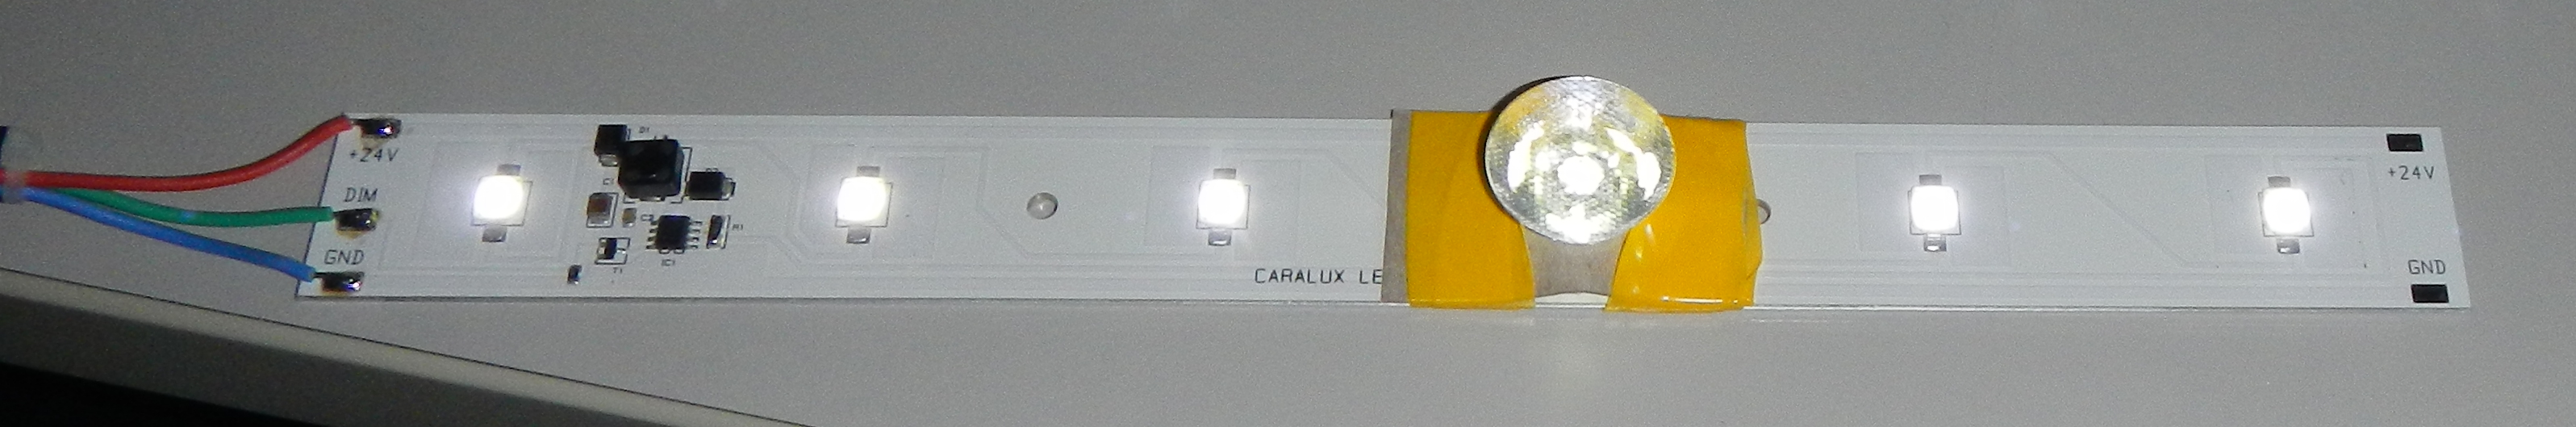
\includegraphics[width=1\hsize]{./images/foto_hardware_ledmodul.png}
\end{center}
\caption[LED-Modul der Firma Caralux mit provisorisch fixierter Optik im Messaufbau, Quelle: Autor]{\label{fotohwledmodul}LED-Modul mit provisorisch fixierter
Optik f\"ur Einsatz im Messaufbau.}
\end{figure}
Die LED-Module sind jeweils mit sechs wei\ss{}en LEDs LUW W5AM-LX-6Q der Firma Osram best\"uck, die eine Farbtemperatur von 6500K aufweisen. Weitere
Informationen zu diesem LED-Typ k\"onnen aus dem zugeh\"origen Datenblatt entnommen werden, welches unter \cite{specled} abgerufen werden kann. Durch die hohe
Leistungsaufnahme der LED-Module sollten diese ohne zus\"atzliche K\"uhlelemente nur f\"ur sehr kurze Zeitr\"aume in Betrieb genommen werden.

Die LED-Module sind so konstruiert das diese mit verschiedenen Optiken versehen werden k\"onnen um die Abstrahlcharakteristik jeder einzelnen LED variieren zu
k\"onnen. Im Messaufbau wurden Messreihen f\"ur die Optiken Titanium-M und Titanium-SS aufgenommen.
\begin{figure}[htb]
\begin{center}
  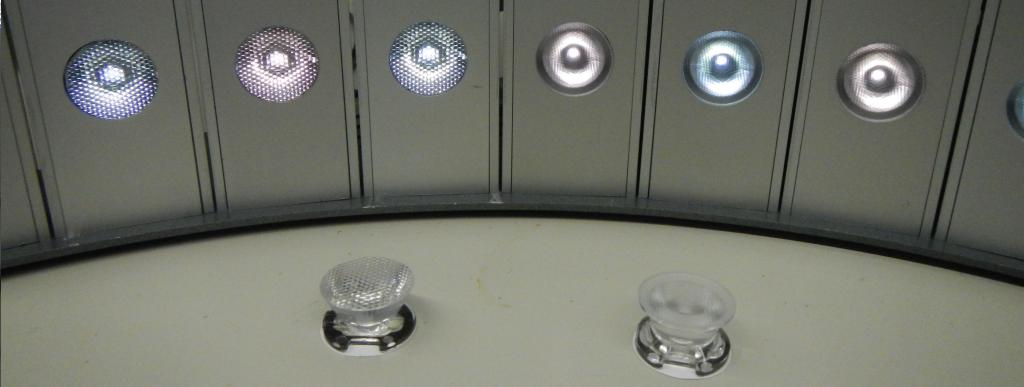
\includegraphics[width=1\hsize]{./images/foto_hardware_optiken.png}
\end{center}
\caption[LED-Optiken, links: Titanium-M, rechts Titanium-SS, Quelle:
Autor]{\label{fotohwoptiken}LED-Optiken, links: Titanium-M, rechts Titanium-SS, Quelle:
Autor}
\end{figure}
Die LED-Optiken besitzen einen Fuss, der an das LED-Modul angepasst ist. Weiterhin sind die LED-Optiken an der Unterseite mit doppelseitigem Kelebematerial
versehen, was eine leichte Fixierung auf dem LED-Modul erm\"oglicht.

\subsection{Mikrocontroller LPC1768}
Den Kern des Projekts bildet die Mikrocontrollerbaugruppe LPC1768 der Firma NXP. Diese Baugruppe basiert auf einem ARM Cortex-M3 

\cite{speclpc1768}

\subsection{PWM-Controller PCA9685}

Der verwendete PCA9685 ist ein programmierbar PWM-Controller mit 16 Kanälen und einer Auflösung von 12 Bit. Angesteuert wird dieser Controller über das Bus-Protokoll I2C. Durch sechs vorhandene Adresspins können bis zu 62 PCA9685 an einem Bus betrieben werden. Des Weiteren ist es möglich alle am Bus befindlichen Controller gleichzeitig über eine All-Call-Adresse anzusprechen sowie zu konfigurieren. Über einen separaten OE-Eingang kann die PWM-Ausgabe komplett an- und abgeschaltet werden.  

\subsubsection{Konfiguration}
Konfiguriert wird der Controller mittels acht Bit großer Register. 

\subsubsection{Ansteuerung}
Wie eingangs beschrieben erfolgt die Ansteuerung über das I2C-Protokoll.

\subsection{Lichtsensor TSL2561}
Sebastian
\subsection{Lichtsensor GeoSys GSLx}
Sebastian
TODO: Bild einf\"ugen: Oszi-Diagramm: Kanal1=PWM-Output PCA9685, Kanal2=GeoSys Sensor-Output (Kurven \"uberlagern um Zusammenhang zu verdeutlichen)

\subsection{Temperatursensor DS18S20}
Marcel

\clearpage
\section{Versuchsanordnung}

\clearpage
\section{Implementierung}
Sebastian

- Pwm Ansteuerung
- Lichtmessung TSL
- Lichtmessung GSLx


\clearpage
\section{Auswertung}
\subsection{Messergebisse}

\clearpage
\section{Schlussbetrachtung}
\subsection{Messergebisse}


%% Tabelle

%\vspace*{1cm}
%\begin{longtable}{p{34mm}>{\columncolor[gray]{0.97}}p{33mm}p{33mm}>{\columncolor[gray]{0.97}}p{33mm}}
%\rowcolor[gray]{.9}Funktion & \textbf{IPCop} & \textbf{IPFire} & \textbf{pfSense}\\
%Lizenz & GPL\cite{GPLLicense} & GPL\cite{GPLLicense} & BSD\cite{FreeBSDLicense}\\
%\rowcolor[gray]{.95}Betriebssystem & Linux & Linux & FreeBSD   \\
%Hardware"-architektur & i386, Cobald, Sparc, PowerPC & i386, AMD64 & i386, AMD64\\
%\caption{Merkmale ausgew\"ahlter Routerdistributionen im Vergleich}
%\label{Merkmale der Routerdistributionen im Vergleich}
%\end{longtable}

\clearpage
\section{Schluss}
Dies ist der Schlussteil. Abschlie\ss{}ende Empfehlung

\clearpage
\section{Glossar}
\begin{description}
 \item[I2C] Prtokoll zur Kommunikation in Ger\"aten
\end{description}

\clearpage
\section{Literatur- und Quellenverzeichnis}

\renewcommand\refname{Literaturverzeichnis}
\begin{thebibliography}{999}

\bibitem{buch_foobar}Michael W. Lucas:  {\sl Absolute BSD (2nd Edition). The Ultimate Guide to FreeBSD.} No Starch Press, 2008,
\\ISBN: 978-1-59327-151-0

\end{thebibliography}

\renewcommand\refname{Quellenverzeichnis}
\begin{thebibliography}{999}

%%\cite{citeverweis}
\bibitem{speci2c}
\url{http://www.nxp.com/documents/user_manual/UM10204.pdf}
\\Abrufbar am 10.03.2013

\bibitem{spec1wire}
\url{http://www.1wire.org}
\\Abrufbar am 10.03.2013

\bibitem{specled}
\url{http://www.osram-os.net/osram_os/CN/Downloads/Solid_State_Lighting/documents/LUW_W5AM_Pb-free_C_final.pdf}
\\Abrufbar am 10.03.2013

\bibitem{specpwm}
\url{http://www.nxp.com/documents/data_sheet/PCA9685.pdf}
\\Abrufbar am 11.03.2013

\bibitem{speclpc1768}
\url{http://www.nxp.com/documents/data_sheet/LPC1769_68_67_66_65_64_63.pdf}
\\Abrufbar am 11.03.2013\end{thebibliography}

\clearpage
\section{Verzichtserkl\"arung}
\thispagestyle{plain}

Hiermit erkläre ich, dass ich die vorliegende Arbeit selbstständig und nur unter Verwendung der angegebenen Literatur und Hilfsmittel angefertigt habe.
Stellen, die wörtlich oder sinngemäß aus Quellen entnommen wurden, sind als solche
kenntlich gemacht.\\

Diese Arbeit wurde in gleicher oder ähnlicher Form noch keiner anderen Prüfungsbehörde vorgelegt.\\\\

Leipzig, \today
\end{document}
%% EOF